\documentclass[conference]{IEEEtran}
\IEEEoverridecommandlockouts
\usepackage{cite}
\usepackage[utf8]{inputenc}
\usepackage[english]{babel}
\usepackage{bookmark}
\usepackage[square,sort,comma,numbers]{natbib}
\usepackage{listings}
\usepackage{url}
\usepackage{wrapfig}
\usepackage{caption}
\usepackage{color}
\usepackage{enumitem}
\usepackage{graphicx}
\usepackage{float}
\usepackage{url}
\def\UrlBreaks{\do\/\do-}
\usepackage{breakurl}
\graphicspath{{images/}}
\usepackage{hyperref}


\def\BibTeX{{\rm B\kern-.05em{\sc i\kern-.025em b}\kern-.08em
T\kern-.1667em\lower.7ex\hbox{E}\kern-.125emX}}

\date{May 13, 2019}

\makeatletter
\let\thedate\@date


\definecolor{codegreen}{rgb}{0,0.6,0}
\definecolor{codegray}{rgb}{0.5,0.5,0.5}
\definecolor{codepurple}{rgb}{0.58,0,0.82}
\definecolor{backcolour}{rgb}{0.95,0.95,0.92}

\lstdefinestyle{mystyle}{
    backgroundcolor=\color{backcolour},   
    commentstyle=\color{codegreen},
    keywordstyle=\color{magenta},
    numberstyle=\tiny\color{codegray},
    stringstyle=\color{codepurple},
    basicstyle=\scriptsize,
    breakatwhitespace=false,         
    breaklines=true,                 
    captionpos=b,                    
    keepspaces=true,                 
    numbers=left,                    
    numbersep=5pt,                  
    showspaces=false,                
    showstringspaces=false,
    showtabs=false,                  
    tabsize=2
}
    
\lstset{style=mystyle}

\begin{document} 
    \title{
        Project Final Report\\[0.2cm]
        \large ELE494-08\\
        \large \thedate\\
        Submitted to: Dr. Shayok Mukhopadhyay
    }

    \author{
        \IEEEauthorblockN{Nasir Khalid}
        \IEEEauthorblockA{B00065082}
        \and
        \IEEEauthorblockN{Yousif Khaireddin}
        \IEEEauthorblockA{B00063618}

    }

    \maketitle

    \section{Objective}

    Develop a robot that will be given it's starting position within a map.
    With this information t will begin planning the path it will take around the map and during it's journey it
    will read the light intensity of the points. As it does this it will be sending back real time data of
    different parameters \& the light intensity at its position. All of this will be visualized so we can watch
    it in real time. Once it's journey is complete it will go back and remain idle at the point which it determined
    to be the brightest.

    \section{Introduction}
    
    Developing a robot to fulfill our objective required us to break down the entire 
    project in to multiple different pieces and try to accomplish all of these different pieces
    independently. Once done our final aim was to combine it all together. These many pieces are
    the following:

    \begin{itemize}
        \item Develop a Robot that can move in a straight line
        \item Integrate multiple different sensors with the Robot
        \item Get the microcontroller to send data wirelessly
        \item Develop the backend/frontend to visualize data
        \item Add Ackerman steering to drive robot to a certain (x, y) co-ordinate
        \item Use complementary filters on our sensors
        \item Add the light intensity measurement\\
    \end{itemize}

    We achieved 6 out of the 7 objectives we aimed for and through this we were able
    to essentially accomplish a great deal of work that lay the foundations for the rest
    of the project.\\

    Through the report we highlight our entire development process starting with obtaining
    our hardware and then assembling it. We discuss the different features and how they 
    were implemented as well as the code used for each.\\

    We also set up a GitHub repository that contains all documentation and code for the project,
    through the commits it is also shown how we distributed work amongst the two of us. This can
    found here (https://github.com/NasirKhalid24/ELE494-08-Project)


    \section{Methodology\\}

    \subsection{Hardware}
    
    For the actual robot chassis and construction, we bought and built the small car
    that can be seen in figure 1 and decided to repurpose it for our project.

    \begin{figure}[H]
        \centering
        \captionsetup{justification=centering}
        \centering
        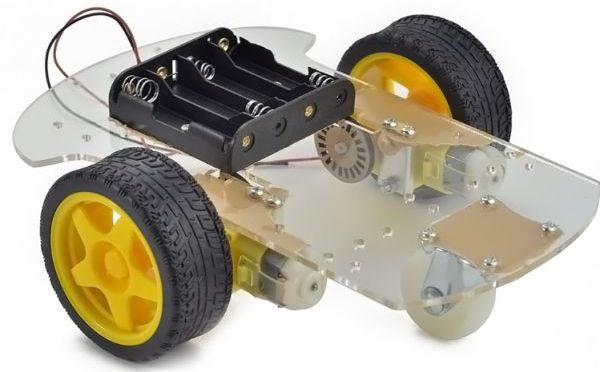
\includegraphics[width=1in]{1.jpg}
        \caption{Robot Chassis, Wheels, \& Motors}  
        \label{1}
    \end{figure}

    To be able to control the direct as well as speed of rotation of each of the
    wheels, we used a Dual H-Bridge which can be seen in figure 2. This was
    adequate since it provided the had the required current rating for the
    motors stall torque current draw.

    \begin{figure}[H]
        \centering
        \captionsetup{justification=centering}
        \centering
        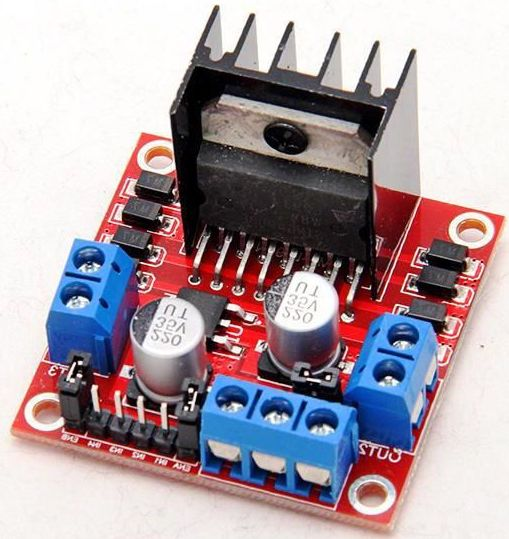
\includegraphics[width=1in]{2.jpg}
        \caption{L298N Dual H-Bridge motor controllers}  
        \label{2}
    \end{figure}

    As for the onboard controller, we had initially started by using a
    regular Arduino; however, once we decided to incorporate the real-time
    tracking of information, we then decided to switch to the NodeMCU that
    can be seen in figure 3. The reason behind this will be explained in the
    following sections.

    \begin{figure}[H]
        \centering
        \captionsetup{justification=centering}
        \centering
        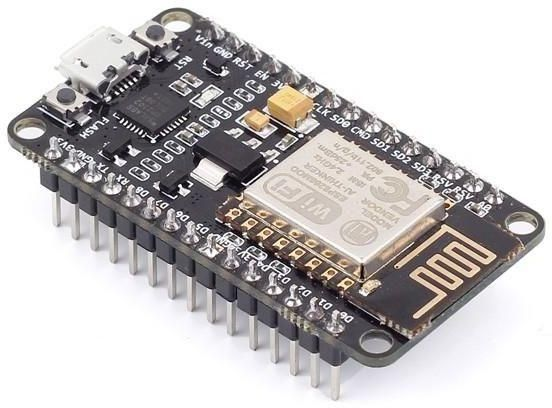
\includegraphics[width=1in]{3.jpg}
        \caption{ESP8266 based NODEMCU microcontroller}  
        \label{3}
    \end{figure}

    Next major piece of hardware required would be the actual accelerometer
    we decided to use. Due to the limited number of ports on the NodeMCU, 
    we had to choose a very small accelerometer that required a maximum of
    three pins. Luckily, we were able to find the one shown in figure 4
    which perfectly meets these criteria.

    \begin{figure}[H]
        \centering
        \captionsetup{justification=centering}
        \centering
        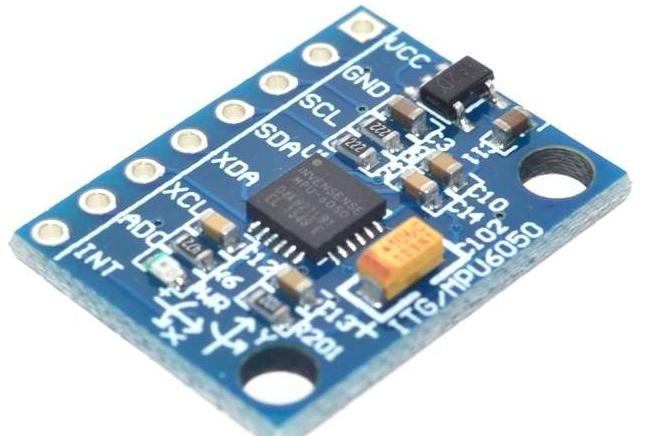
\includegraphics[width=1in]{4.png}
        \caption{MPU6050 3 axis accelerometer/gyroscope}  
        \label{4}
    \end{figure}

    As previously discussed, we hoped to combine the reading of the accelerometer
    with that of an encoder. For this, we decided to buy the encoder that can
    be seen in figure 5. The speed measuring module attaches to the rotary
    encoder and emits a pulse periodically which can be used to give an
    estimate of speed.

    \begin{figure}[H]
        \centering
        \captionsetup{justification=centering}
        \centering
        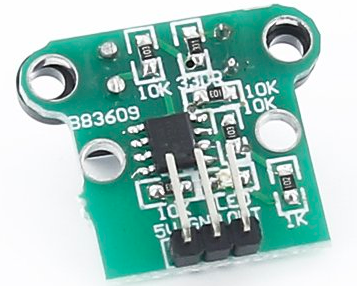
\includegraphics[width=1in]{5.png}
        \caption{HC-020K Speed Measuring Module and Rotary Encoder}  
        \label{5}
    \end{figure}

    Of course, for our actual project to have taken place we would require
    something that can give us an understanding of light intensity in a certain
    area. For this, we decided to use the LDR sensor shown in figure 6.

    \begin{figure}[H]
        \centering
        \captionsetup{justification=centering}
        \centering
        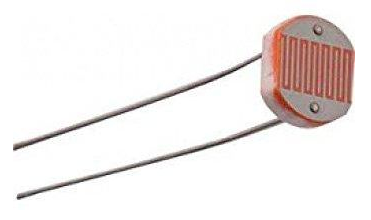
\includegraphics[width=1in]{6.png}
        \caption{Photoresistor LDR CDS 5mm}  
        \label{6}
    \end{figure}

    Finally, to power everything, we decided to use the power bank shown in
    figure 7 due to availability.

    \begin{figure}[H]
        \centering
        \captionsetup{justification=centering}
        \centering
        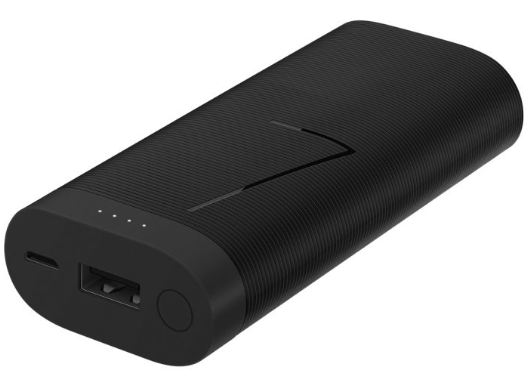
\includegraphics[width=1in]{7.png}
        \caption{Huawei 6700 mAH power bank}  
        \label{6}
    \end{figure}

    \subsection{Robot Assembly}

    Once all the parts have been tested separately, it was time to
    combine everything together to build the final robot. This took some
    time to ensure that all the wiring and soldering was correct and
    that the all the parts were oriented correctly and still operating
    as required. The final construction can be seen in the figures below.

    \begin{figure}[H]
        \centering
        \captionsetup{justification=centering}
        \centering
        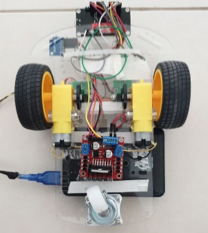
\includegraphics[width=2in]{8.png}
        \caption{Bottom view of Robot}  
        \label{6}
    \end{figure}
    
    \begin{figure}[H]
        \centering
        \captionsetup{justification=centering}
        \centering
        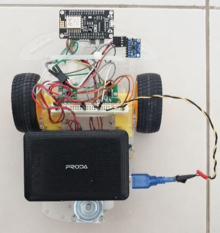
\includegraphics[width=2in]{9.png}
        \caption{Top view of Robot}  
        \label{6}
    \end{figure}

    \subsection{Position Estimation}

    Regarding the actual localization of the robot, we decided to
    try and construct a complementary filter and combine our encoder and
    accelerometer readings for a better estimate of position. This is
    be done by reading each of them separately, changing their readings
    into position through the required integrations necessary, then performing
    a weighted average to combine the results. The difficulty here
    is trying to understand which of the two sensors performs better so as
    to properly choose the weights.\\

    \subsection{Robot Movement}

    Once the robot has successfully learned how to locate its position
    relative to an axis, it must also learn to move to any specific point,
    as required. For this, we decided to implement Ackerman’s steering since
    it eliminated the need for any PID gain tuning and should still provide
    satisfactory results. It is important to note that the route taken from
    point A to point B will be completely random and that there’s no guarantee
    that it will be the same every time. For our application, however, this
    was not an issue.\\

    \subsection{Real-time Communication}

    Finally, as for the real-time aspect of the project, we connect
    to the NodeMCU wirelessly and execute a function that will continuously
    have it transfer information about the robots parameters and the 
    backend then plots this
    information in real-time. This was the reason we decided to switch from
    an Arduino to the NodeMCU. Its inbuilt functionality which allows it to
    connect to an existing WiFi network and easily transmit
    data will vastly facilitate the transfer of data between the robot and our server.\\

    \subsection{Experimentation}

    \subsubsection{Parts Operation}

    ~~\\Once all the parts have arrived, it was essential to test that each of
    them was actual operating properly. For this, we ensured to construct different
    testing procedures that will help us ensure that the operation of each part is
    sensible and appropriate and this can be seen in the following.\\

    \paragraph{Motors and Motor Driver}

    ~~\\For this we started by applying a voltage to the motors ensuring their proper
    rotation in both directions. We then varied these voltage inputs to ensure that
    the motors are in fact responding to changes in voltage values. This is
    important as it enables us to perform speed control.\\
    
    Once that has been completed, we then connected the motors to the motor driver
    and fed the motor drive the required pin configurations to turn the motors in
    both directions as well as ensured to test that different inputs to the enable
    pins would cause a change in motor speed; thus, further confirming our ability
    to perform speed control. The setup for these tests can be seen in figure 10.\\

    \begin{figure}[H]
        \centering
        \captionsetup{justification=centering}
        \centering
        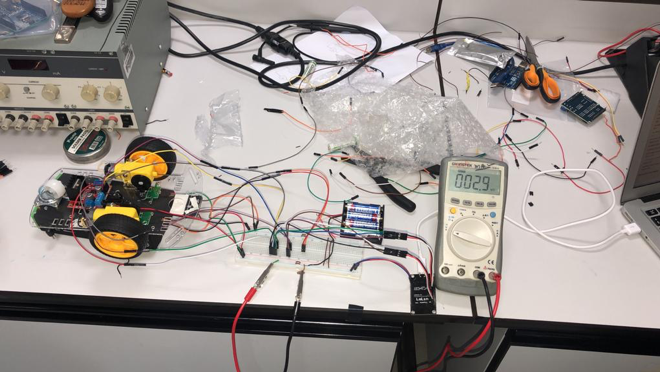
\includegraphics[width=2.5in]{10.png}
        \caption{Preliminary Testing}  
        \label{6}
    \end{figure}

    \paragraph{Sensors}

    ~~\\One of the first test we made was to ensure that accelerometer values were
    sensible. This was done by keeping it constant in all directions and placing
    a different face pointing downwards. The goal here was to ensure that whenever
    a specific side faced downwards, its acceleration was roughly 9.81 m/s2 while
    everything else was roughly 0 m/s2 (no motion). The code for the accelerometer is
    quite large and therefore it is included in the Appendix along with the other
    robot code. The basic operation
    was I2C based and we would the register values from the sensor and then multiply
    them by 9.81 to get them in m/s2\\

    Once that has been completed, it was important to test the encoder readings,
    this was done by manually rotating the wheel through 1 rotation and ensuring
    that the counter value reaches 20. This is the case since there are 20 slots
    in our rotary encoder. After the test we then implemented code to get to read
    the encoder value and convert it to revolutions per second. This is shown below:

\begin{lstlisting}[language=C++, caption=Encoder Code]
//obtain the speed of wheels in revolutions/sec 
//using the count values from the interrupt functions
//20 is the number of slits in the encoder 
rev1 = count1/(20*ts);
rev2 = count2/(20*ts);

//change these speeds into m/s for each wheel
v1 = rev1*2*PI*radius;
v2 = rev2*2*PI*radius;

//obtain actual robot speed
v_actual = (v1 + v2)/2;\end{lstlisting}

    The radius was measured and defined in the beginning of the code as 0.032955 m. Along
    with the PI constant. 'ts' is the timestep betwen loops for testing we kept it as a small
    value based on our delays but afterwards we wrote code to get a more accurate value and
    this is shown in later sections.\\

    \paragraph{Data Transfer}

    ~~\\The next major section we had to test is the ability for us to connect to the
    NodeMCU wirelessly and extract data in real-time. This was done by running a
    loop that sent some values over to the computer and cross checking that these
    values were as expected. This is illustrated in figure 11.

    \begin{figure}[H]
        \centering
        \captionsetup{justification=centering}
        \centering
        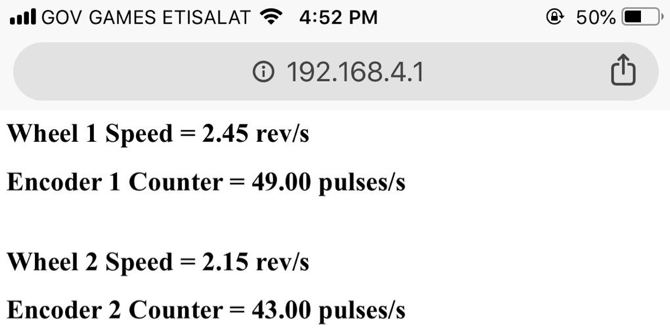
\includegraphics[width=2.5in]{11.png}
        \caption{Data Transfer Test}  
        \label{6}
    \end{figure}

    \subsubsection{Calibration}

    ~~\\Due to mismatches in design motor design, imperfect weight distributions,
    as well as a number of other factors, we were required to find a ratio between
    the wheel pwm inputs that would ensure the robot behaves as required. Without
    this step, feeding both motors the same voltage will cause the car to tilt
    towards one direction rather than go straight. For this, a number of tests and
    trials were done while varying a scale factor until we found the correct one
    which will ensure proper movement. The code showing this factor can be seen below.

\begin{lstlisting}[language=C++, caption=Wheel Calibration Code]
//Note: The 0.9 factor is just used for calibration since 
//motors aren't identical
analogWrite(EN1, pwm_l*0.9);  
analogWrite(EN2, pwm_r);\end{lstlisting}

    \subsubsection{Speed Control}

    ~~\\Once the above has been completed, we then moved on to running a number
    of tests to ensure that we can control each motors speed through altering
    the PWM input which will in turn give us the ability to turn left and right
    as required.\\

    \subsubsection{Position Estimation}

    ~~\\As previously discussed, to properly detect the position of our robot,
    we decided to combine the readings of an accelerometer and an encoder using
    a complementary filter. In this section, we were faced by a number of choices.
    One of the first choices we had to make is which of the following two methods
    to utilize when designing the filter:\\

    \paragraph{Method 1}

    \begin{itemize}
        \item Integrate the accelerometer once
        \item Merge that reading with the encoder speed to obtain a speed estimate
        \item Integrate the weighted average to obtain a measurement of position\\
    \end{itemize}

    \paragraph{Method 2}

    \begin{itemize}
        \item Integrate the accelerometer twice
        \item Integrate the encoder once
        \item Merge the results using a weighted average to obtain a position estimate.\\
    \end{itemize}

    One way to resolve this is by just choosing the method that has the least
    number of integrations before yielding the result. This argument is purely based
    on the discussions we had in class discussing the inaccuracies and problems that
    direct integration can result in. However, as can be seen above both methods need
    at least two integrations so they are identical in this aspect.\\

    To resolve this, we decided to implement both options to see which would yield
    better results. Unfortunately, since both our encoder as well as our accelerometer
    readings were extremely inaccurate and very noisy to begin with, neither of them
    gave us any concrete results, so we decided to just go with method 2 since its
    slightly more convenient because the final output of the filter is directly position.\\

    One important thing to note is that when we had initially started testing, we
    initially assumed a constant timestep of 100ms for the integrations which is
    very wrong especially since at each loop, depending on certain values there are
    specific delays placed which can significantly contribute to this timestep.
    For this, we later ensured to internally measure this timestep and fix these
    wrong assumptions. This was done using the code shown below:

\begin{lstlisting}[language=C++, caption=Time Step Code]
//obtaining the timestep between loops  
ts = (millis() - tremove)/1000;  
tremove = millis();\end{lstlisting}
    
    We would save the current time in the tsremove function and once the loop would
    end we would get the time taken by subtracting the initial time from the current time
    and saving it in the 'ts' parameter. This was used during the integration.\\

    Of course, the next choice we had to make was choosing the weights of this filter.
    To do this, we varied them across several different cases including some extremes
    of (0.95 \& 0.05) just to see the behavior of the car. Although still not great due
    to the extremely faulty hardware, our best results were obtained using 0.7 on the
    encoder and 0.3 on the accelerometer. This kind of makes sense since the
    accelerometer undergoes two accelerations while the encoder only goes through one.\\

    Shown below is code that was used to integrate as well as the complementary filter code:

\begin{lstlisting}[language=C++, caption=Integration Code and Complementary Filter Code]
//obtaining positions using integration of encoder velocity 
x_1= x_1+ ts*v_actual*cos(theta);
y_1= y_1+ ts*v_actual*sin(theta);
theta = theta + ts*w;

//obtaining velocities using integration of accelerometer values
Vx = Vx + ts*Ax;
Vy = Vy + ts*Ay;

//obtain position using second integration of accelerometer
x_2= x_2+ ts*Vx;
y_2= y_2+ ts*Vy;

//obtaining an estimate of position using complementary filter  
x = x_1 * w1 + x_2 * w2;
y = y_1 * w3 + y_2 * w4;\end{lstlisting}

    Ax and Ay are the accelerations in the x and y direction respectively, where as the v actual,
    is the speed of the robot. The theta and w values are obtained from Ackermans steering which
    is discussed next.\\

    \subsubsection{Ackerman’s Steering}

    ~~\\Even though our estimate of position was very wrong, we still decided to carry
    on and build the code required for Ackerman’s steering. In this section we had
    to decide the choice of h and K. Initially, we had chosen a h value of 0.5 and
    a K matrix of [0.5 0 ; 0 0.5].\\

    As per our discussion with Dr. Shayok, we have been told that a larger h and a
    smaller K would lead to a smooth convergence. For this, we then ended up with
    an h of 1 and a K of [0.2 0; 0 0.2].\\
    
    Of course since our position estimates were not correct by any means, we were
    never able to verify the actual workings of this code; however, by cross
    referencing with other online sets of code as well as our homework solutions,
    we are confident it would. This is the case since the robot does react to errors
    as can be seen in the results section of this report where as the x and y values
    get further and further from the point they are intended to reach, the wheel
    velocities get higher and higher. This indicates that there really is a reaction
    to error. Shown below is the code used for Ackerman’s steering:\\

\begin{lstlisting}[language=C++, caption=Ackerman’s Steering Code]
//implementing ackermans steering
xh = x + h*cos(theta);
yh = y + h*sin(theta);

e1 = xh - xr;
e2 = yh - yr;

v = (k1*cos(theta) + k2*sin(theta))*e1;
w = ((-k1*sin(theta)/h) + (-k2*cos(theta)/h))*e2;\end{lstlisting}


    \subsubsection{Data Transfer and Visualization}

    ~~\\To have the robot transfer data to our computer in real time we first had to
    set up the NODEMCU device to connect to a WiFi network through which it could send
    data. To do this in our code first gave the robot the WiFi credentials as string
    variables and then asked in to connect to the network in the setup function. If the
    robot disconnects in the main loop it also attempts to reconnect. The robot is also
    given an IP address which corresponds to our server IP address that will be discussed
    next. Shown below is code for the credentials and connection:

\begin{lstlisting}[language=C++, caption=Robot Connection Code]
// Connection credentials
const char* WIFI_NAME = "Daedalus";
const char* WIFI_PASS = "flightoficarus";
const char* host = "192.168.43.177";

void Connect2Wifi(){
    WiFi.mode(WIFI_STA);
    WiFi.disconnect();
    delay(100);
    
    WiFi.begin(WIFI_NAME, WIFI_PASS);
    delay(4000);}\end{lstlisting}

    The Robot connects to the Daedalus network which is a mobile hotspot network because
    the AUS network requires additional login information that the chip cannot be configured
    with. The host given to the computer is the server address for our backend where we
    process the data sent and host the webpage used to display the real time results. Once
    the Robot has collected the required information it then sends the data as a POST request
    to the 'host' IP address that it was provided. The function to send data has multiple parameters,
    one for each of the different variables. In the function these variables are then sent.
    The whole function can be seen below:

\begin{lstlisting}[language=C++, caption=Send Data Function]
void SendData(double X,double Y, double VL,double VR,double PWM_L,double PWM_R,double TS, double E1, double E2, double REV1, double REV2, double V1, double V2, double V_ACTUAL, double AX, double AY, double AZ, double T, double OX, double OY, double OZ){
    HTTPClient http;
    http.begin("http://" + String(host) + ":5000/data");
    http.addHeader("Content-Type", "application/x-www-form-urlencoded");
    http.POST(
        "x=" + String(X) + "&"
        "y=" + String(Y) + "&"
        "vl=" + String(VL) + "&"
        "vr=" + String(VR) + "&"
        "pwm_l=" + String(PWM_L) + "&"
        "pwm_r=" + String(PWM_R) + "&"
        "TS=" + String(TS) + "&"
        "E1=" + String(E1) + "&"
        "E2=" + String(E2) + "&"
        "REV1=" + String(REV1) + "&"
        "REV2=" + String(REV2) + "&"
        "V1=" + String(V1) + "&"
        "V2=" + String(V2) + "&"
        "V Actual=" + String(V_ACTUAL) + "&"
        "AX=" + String(AX) + "&"
        "AY=" + String(AY) + "&"
        "AZ=" + String(AZ) + "&"
        "T=" + String(T) + "&"
        "OX=" + String(OX) + "&"
        "OY=" + String(OY) + "&"
        "OZ=" + String(OZ)
        );
    http.writeToStream(&Serial);
    http.end();
}\end{lstlisting} 
    
    Our backend server is written in Javascript. It uses NodeJS which allows us to execute
    the Javascript files. It uses Express to host a server and Websockets to help send data
    from server to the front end website. The code snippet shown below illustrates that when
    the root of the server ('/') is visited on a webpage we return the 'index.html' page.
    The second function shows that when a POST request is sent to '/data' we use websockets
    to emit the data as a variable called 'data' as well as log the data on the console.

\begin{lstlisting}[language=C++, caption=Server Code Snippet]
app.get('/', function(req, res){
    res.sendFile(express.static(__dirname + '/src/index.html'));
});

app.post("/data", function(req, res) {
    io.sockets.emit("data", req.body);
    console.log(req.body)
    res.send({});
});\end{lstlisting}

    The address for the server is fixed and is the same one that is saved as 'host' on the microcontroller. We
    have discussed how the backend process data and emits it, as well as how it serves the index.html
    front end. Now we will discuss how the 'index.html' gets the emitted data and converts it to a 
    graph. For the front end we created a basic html page that has a heading and for each graph
    it has a 'div' element block which contains the title and a spot for the graph. Shown below
    is an example of the 'div' block

\begin{lstlisting}[language=C++, caption=HTML Graph Div Snippet]
<div id="Graph of Y" class="Graph Box">
    <h2>Graph of Y (Time vs Position)</h2>
    <div id="y"></div>
</div>\end{lstlisting}

    In this block we contain a 'div' element under the 'h2' heading element, this is where we display
    the graph. Each of them have a seperate and unique 'id' parameter. The 'id' is also the same as the
    ID's used in the SendData function shown in Listing 3. For example the 'id' above is 'y' and in the
    SendData function we also send 'Y' with the id of 'y'.\\

    Javascript code is also used in the HTML page to receive the emitted data and create a graph.
    For graphing we use a library called 'Rickshaw' which takes away much of the extra code needed to
    generate the figure. In the Javscript file we start by creating a class called 'Data', this class
    is given 4 main parameters in its constructor function:\\

    \begin{itemize}
        \item Width of Graph
        \item Height of Graph
        \item 'id' of the corresponding div
        \item Timestep\\
    \end{itemize}

    The entire code for the created 'Data' class can be found in the appendix and it also shows the different
    functions made for the classes that it uses to create the graph and extract data. The parameters 
    passed in the constructor are used to create the graph itself and also used to identify which variable
    it needs to pull from the entire data being emitted. Shown below is a snippet of the constructor for the
    Data Object.
    
\begin{lstlisting}[language=C++, caption=Data Class Constructor]
class Data{
constructor(width, height, id, timestep) {
    this.height = height;
    this.width = width;
    this.name = id
    this.data = [{x: 0, y: 0}];
    this.graph = this.makeGraph();
    this.x = this.makeXAxis();
    this.y = this.makeYAxis();
    this.created = this.createGraph()
    this.timestep = timestep;
}\end{lstlisting}
    
    The data for the graph is defined as an array which contains an object at each index. The object at each
    index is given of the form '\{x: X value, y: Y value\}' where the X value and Y value are the points on the 
    graph. When we extract new data we call the function below and pass it the data as a parameters

\begin{lstlisting}[language=C++, caption=Extract Values Function]
extractValues(d){
    this.data.push(
        {x: this.data.length * this.timestep,
        y: parseFloat(d[`${this.name}`])}
    )
    this.updateGraph()
}\end{lstlisting}
    
    Here we multiply the timestep by the array index to get the time value for the X, for the Y value we
    simply extract the data from the passed to the function where the key for the data is the same as the 'id' passed
    to the constructor. The data is the parsed as a float value. The final x and y object is then pushed to the data array
    and we then update the graph.\\


    Since the 'id' of the variable is same on the
    HTML page and in the ID of the POST data send by the robot, we can use the single ID to identify where to put the Graph
    on the webpage as well as which variable it is from the entire data. Shown below is some code where
    we instantiate different objects of the 'Data' class for the variables we want to extract from the data recieved,
    we then call the 'extractValues' function of these objects inside the listener, the listener function gets called when
    the backend emits "Data". In it we call the extractValues function for each object which extract the respective data
    from the entire data recieved. In the extractValues function we also call the update graph function for the
    object and this is what updates the graph everytime we recieve data.

\begin{lstlisting}[language=C++, caption=Front End Data Listener]
x = new Data(400, 240, 'x', 0.5);
y = new Data(400, 240, 'y', 0.5);
vl = new Data(400, 240, 'vl', 0.5);
vr = new Data(400, 240, 'vr', 0.5);
v1 = new Data(400, 240, 'V1', 0.5);
v2 = new Data(400, 240, 'V2', 0.5);
v = new Data(400, 240, 'V Actual', 0.5);
ax = new Data(400, 240, 'AX', 0.5);
ay = new Data(400, 240, 'AY', 0.5);
az = new Data(400, 240, 'AZ', 0.5);

socket.on('data', function (data) {
    x.extractValues(data)
    y.extractValues(data)
    vl.extractValues(data)
    vr.extractValues(data)
    v.extractValues(data)
    v1.extractValues(data)
    v2.extractValues(data)
    ax.extractValues(data)
    ay.extractValues(data)
    az.extractValues(data)
});\end{lstlisting}

    The code for the creation of the graphs and their x,y axes is in the appendix due to its length but in it we pass the
    'id' to the graph so it can figure out which element to display itself in on the HTML page, we also pass it the data as a
    variable. The function to create the graph returns a Graph object and this object has an inbuilt update function which is called
    whenever we want to update the graph.

    We also style our front end using some basic CSS to center the elements. The final web page looks as shown below:

    \begin{figure}[H]
        \centering
        \captionsetup{justification=centering}
        \centering
        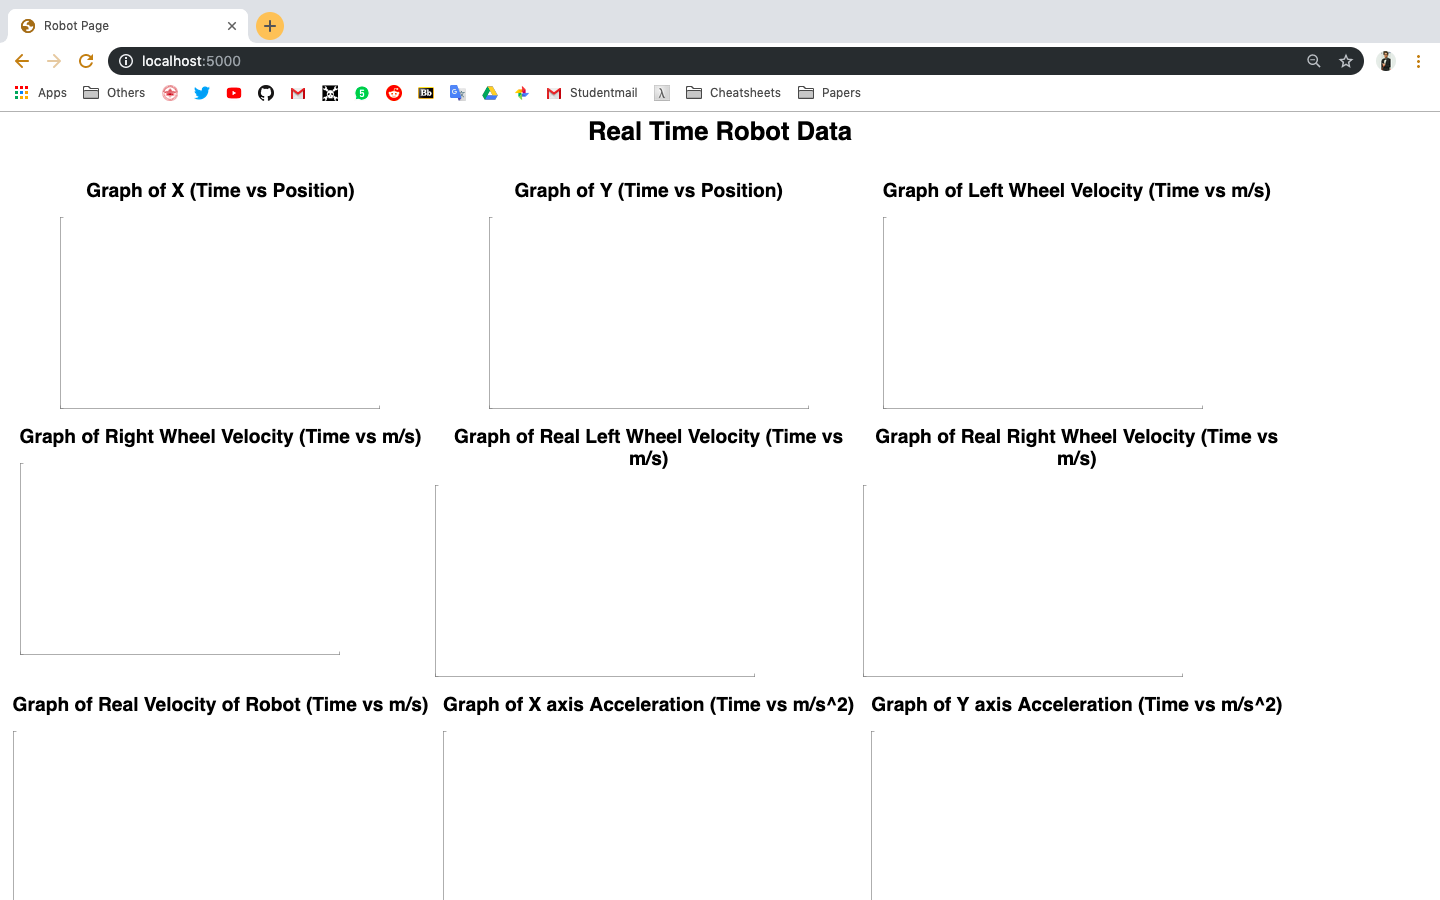
\includegraphics[width=3.8in]{15.png}
        \caption{Webpage without Data}  
        \label{6}
    \end{figure}

    \begin{figure}[H]
        \centering
        \captionsetup{justification=centering}
        \centering
        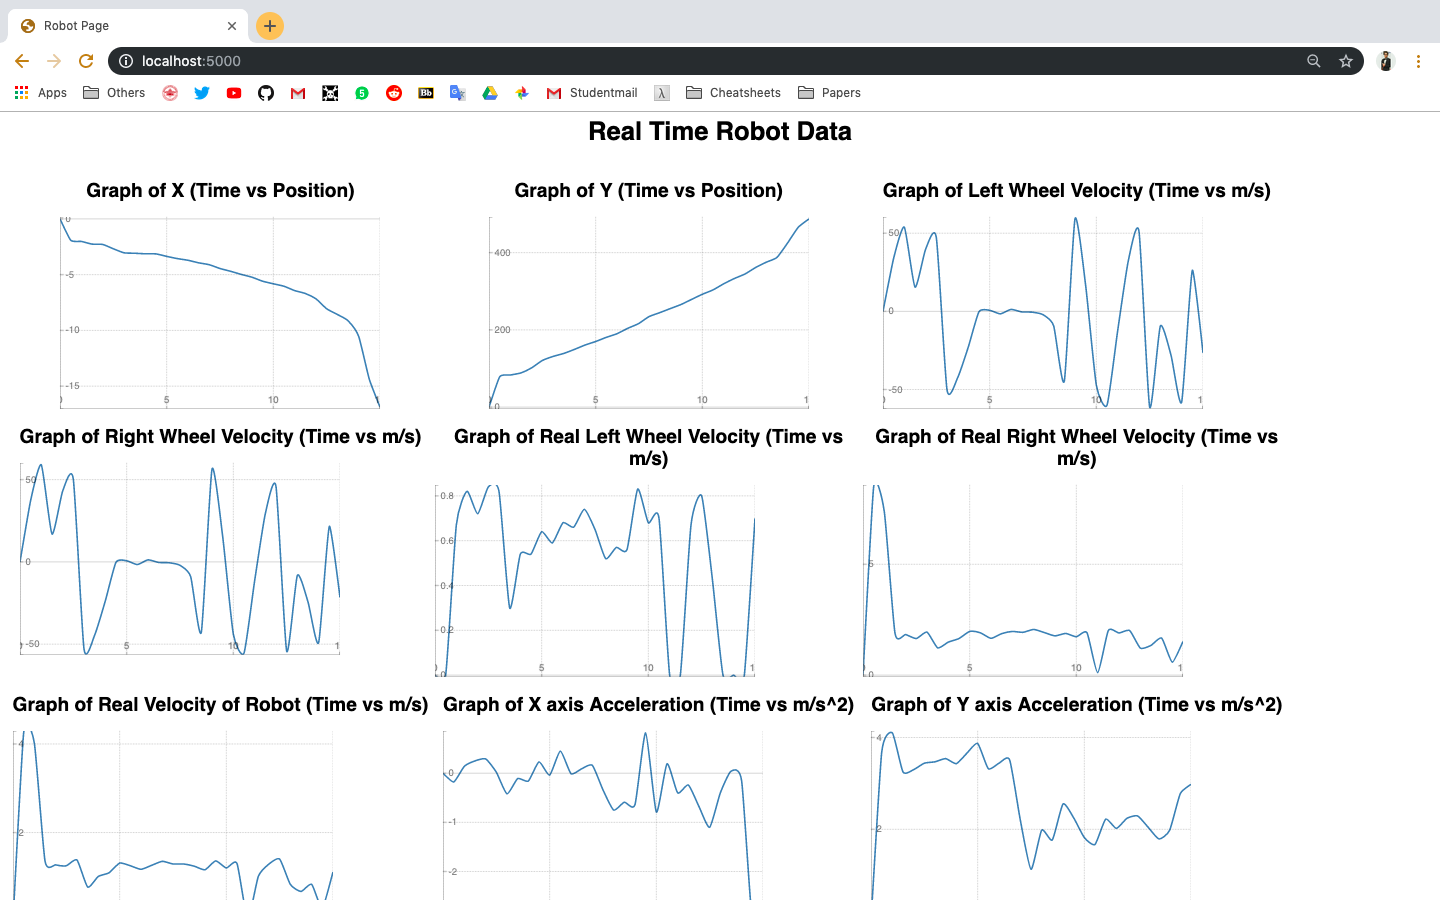
\includegraphics[width=3.5in]{16.png}
        \caption{Webpage with Data}  
        \label{6}
    \end{figure}

    \section{Results}

    Since we had only gotten to building Ackerman’s steering and the complementary,
    there wasn’t much we could show in terms of results. However, as can be seen in
    the plots below we are definitely tracking the values the robot is sending in
    real-time and are accurately plotting them as time passes. In this run, the
    robot was required to go to point (200, 200) which it obviously did not. Had 
    he complementary filter output been somewhat accurate we strongly believe that
    it would’ve been possible

    \begin{figure}[H]
        \centering
        \captionsetup{justification=centering}
        \centering
        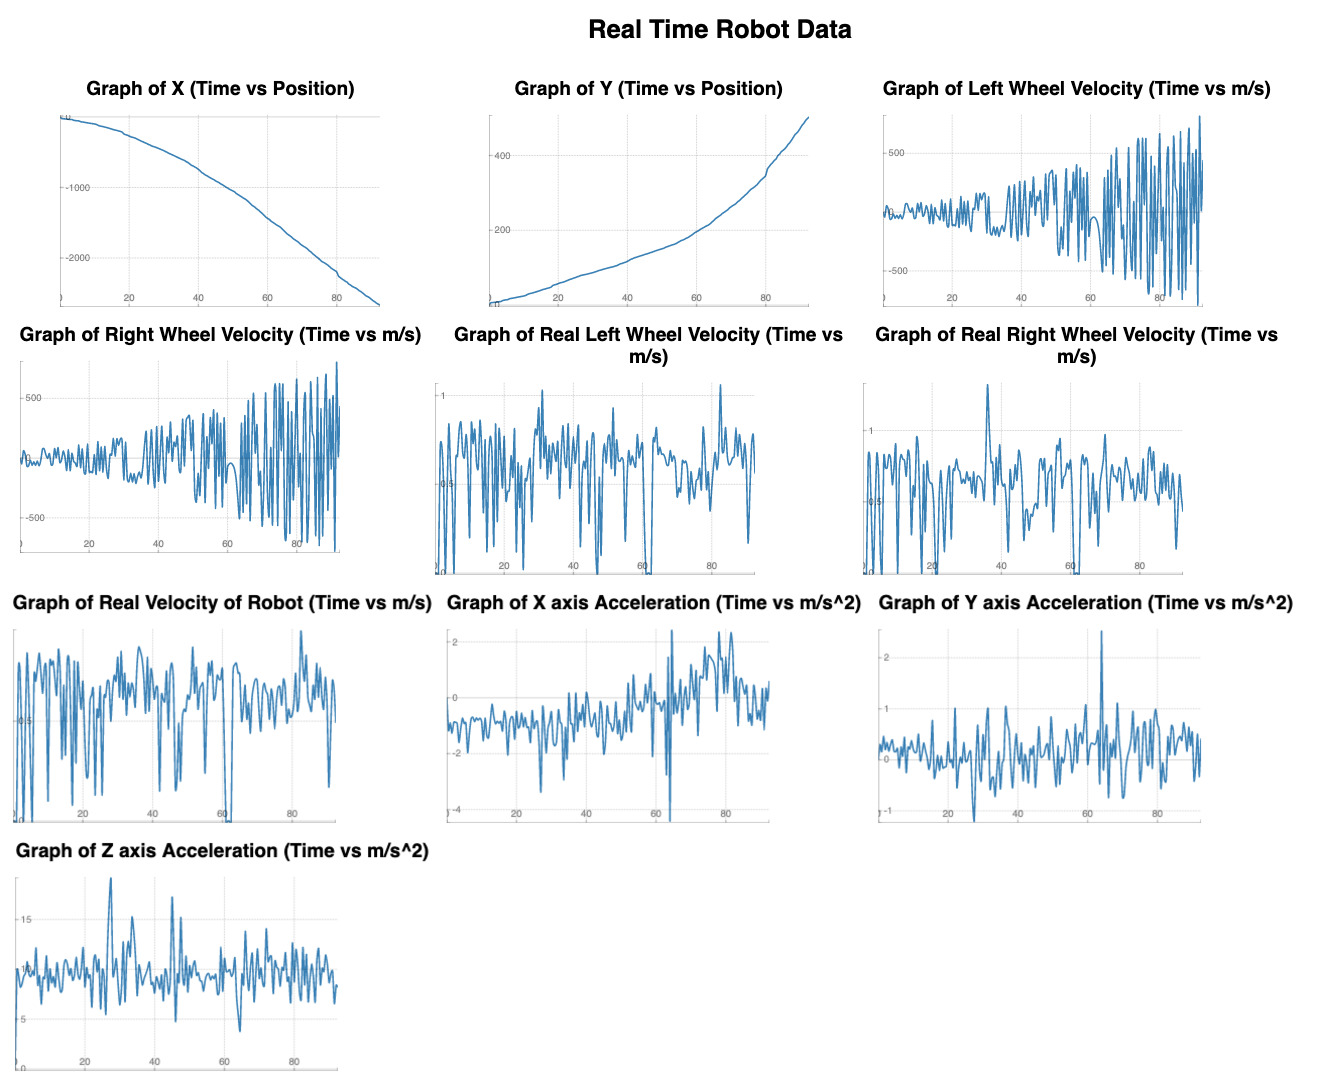
\includegraphics[width=3.5in]{14.jpg}
        \caption{Results of Steering to (200, 200)}  
        \label{6}
    \end{figure}

    This image is also available in the last section of the appendix in much larger resolution.
    \section{Conclusion}

    Through our project we were fortunate enough to be able to work with hardware and software
    that was new to us and allowed us to learn some of the fundamentals of how to develop an
    autonomous robotic system. Although we were note one hundred percent successful we believe
    that we laid the groundwork for developing on top of our existing project as well
    as learning how to develop a new system from scratch. Working with the multitude of sensors
    and implementing the theoretical formulas as code was a challenge that we had not faced before
    and completing the real time display was a novel feature because from our research we were
    not able to find systems online that do this with the same configuration that we used in our
    system. 

    \pagebreak
    \onecolumn 
    \appendix
    
    \section{Robot Code}

\begin{lstlisting}[language=C++, caption=Robot Code]
#include <ESP8266WiFi.h>
#include <WiFiClient.h>
#include <ESP8266WebServer.h>
#include <Wire.h>
#include <ESP8266HTTPClient.h>
#include <time.h>

#define PI 3.1415926535897932384626433832795

//PIN LAYOUT
//EN1 --> D3
//IN1 --> RX
//IN2 --> TX
//IN3 --> D0
//IN4 --> D7
//EN2 --> D4

//ENC1 -->D1
//ENC2 --> D6

// D8 IS BAD. DO NOT USE!

//Pin Definitions
#define ENCODER1 5 //[D1]
#define ENCODER2 12 //[D6]

#define EN1  0  //[D3]
#define IN1  3  //[RX]
#define IN2  1 //[TX]

#define EN2  2 //[D4]
#define IN3  16 //[D0]
#define IN4  13 //[D7] 

#define PI 3.1415926535897932384626433832795
#define radius 0.032955

//requirements to run robot
double count1 = 0;
double count2 = 0;
double rev1 = 0;
double rev2 = 0;
double v1, v2, v_actual;
double ts = 0;
double tremove = 0;
bool flag_p_l = 1;
bool flag_p_r = 1;


//requirements to run ackremenas steering
#define h 1
#define k1 0.2
#define k2 0.2
#define l 0.157
#define w1 0.3
#define w2 0.7
#define w3 0.3
#define w4 0.7

//initial conditions

double x_1= 0;
double x_2= 0;

double y_1= 0;
double y_2= 0;

double Vx = 0;
double Vy = 0;

double x = 0;
double y = 0;
double theta = 0;

double v = 0;
double w = 0;

double xh = 0;
double yh = 0;

double e1 = 0;
double e2 = 0;

double vl = 0;
double vr = 0;

double pwm_l = 0;
double pwm_r = 0;


//final point
double xr = 200;
double yr = 200;


// Connection credentials
const char* WIFI_NAME = "Daedalus";
const char* WIFI_PASS = "flightoficarus";
const char* host = "192.168.43.177";

// Select SDA and SCL pins for I2C communication 
const uint8_t scl = 4; //[D2]
const uint8_t sda = 14; //[D5]

// MPU6050 Slave Device Address
const uint8_t MPU6050SlaveAddress = 0x68;

// sensitivity scale factor respective to full scale setting provided in datasheet 
const uint16_t AccelScaleFactor = 16384;
const uint16_t GyroScaleFactor = 131;

// MPU6050 few configuration register addresses
const uint8_t MPU6050_REGISTER_SMPLRT_DIV   =  0x19;
const uint8_t MPU6050_REGISTER_USER_CTRL    =  0x6A;
const uint8_t MPU6050_REGISTER_PWR_MGMT_1   =  0x6B;
const uint8_t MPU6050_REGISTER_PWR_MGMT_2   =  0x6C;
const uint8_t MPU6050_REGISTER_CONFIG       =  0x1A;
const uint8_t MPU6050_REGISTER_GYRO_CONFIG  =  0x1B;
const uint8_t MPU6050_REGISTER_ACCEL_CONFIG =  0x1C;
const uint8_t MPU6050_REGISTER_FIFO_EN      =  0x23;
const uint8_t MPU6050_REGISTER_INT_ENABLE   =  0x38;
const uint8_t MPU6050_REGISTER_ACCEL_XOUT_H =  0x3B;
const uint8_t MPU6050_REGISTER_SIGNAL_PATH_RESET  = 0x68;

int16_t AccelX, AccelY, AccelZ, Temperature, GyroX, GyroY, GyroZ;
double Ax, Ay, Az, T, Gx, Gy, Gz;

void High_Callback() {
    count1 += 1;
}
void Low_Callback() {
    count2 += 1;
}

void setup() {
    
    Serial.begin(115200);
    Serial.print("STARTED ROBOT");
    
    //Connect to WiFi
    Connect2Wifi();
    
    // Initialize MPU
    Wire.begin(sda, scl);
    MPU6050_Init();

    //Defining PIN directions
    pinMode(EN1, OUTPUT);
    pinMode(IN1, OUTPUT);
    pinMode(IN2, OUTPUT);
    pinMode(EN2, OUTPUT);
    pinMode(IN3, OUTPUT);
    pinMode(IN4, OUTPUT);
    pinMode(ENCODER1, INPUT);
    pinMode(ENCODER2, INPUT);
    
    delay(1000);

    analogWrite(EN1, 1024*0.9);
    analogWrite(EN2, 1024);
    digitalWrite(IN1, LOW);
    digitalWrite(IN2, HIGH);
    digitalWrite(IN3, HIGH);
    digitalWrite(IN4, LOW);
    
    attachInterrupt(digitalPinToInterrupt(ENCODER1), High_Callback, RISING);
    attachInterrupt(digitalPinToInterrupt(ENCODER2), Low_Callback, RISING);
}

void loop(){

    if(WiFi.status() != WL_CONNECTED){
    Connect2Wifi();
    }

    //obtaining the timestep between loops
    ts = (millis() - tremove)/1000;
    tremove = millis();
    
    //obtain the speed of wheels in revolutions/sec using the count values from the interrupt functions 
    rev1 = count1/(20*ts);
    rev2 = count2/(20*ts);

    //change these speeds into m/s for each wheel
    v1 = rev1*2*PI*radius;
    v2 = rev2*2*PI*radius;

    //obtain actual robot speed
    v_actual = (v1 + v2)/2;

    
    //obtaining positions using integration of encoder velocity 
    x_1= x_1+ ts*v_actual*cos(theta);
    y_1= y_1+ ts*v_actual*sin(theta);
    theta = theta + ts*w;
    
    
    //reset counter values in preperation for next v measurement
    count1 = 0;
    count2 = 0;
    
    //obtain accelerometer and gyroscope values 
    Read_RawValue(MPU6050SlaveAddress, MPU6050_REGISTER_ACCEL_XOUT_H);
    //divide each with their sensitivity scale factor
    Ax = (double)AccelX*9.81/AccelScaleFactor;
    Ay = (double)AccelY*9.81/AccelScaleFactor;
    Az = (double)AccelZ*9.81/AccelScaleFactor;
    T =  (double)Temperature/340+36.53;         //temperature formula
    Gx = (double)GyroX/GyroScaleFactor;
    Gy = (double)GyroY/GyroScaleFactor;
    Gz = (double)GyroZ/GyroScaleFactor;

    //obtaining velocities using integration of accelerometer values
    Vx = Vx + ts*Ax;
    Vy = Vy + ts*Ay;

    //obtain position using second integration of accelerometer
    x_2= x_2+ ts*Vx;
    y_2= y_2+ ts*Vy;

    //obtaining an estimate of position using complementary filter  
    x = x_1 * w1 + x_2 * w2;
    y = y_1 * w3 + y_2 * w4;
    
    //implementing ackremans steering
    xh = x + h*cos(theta);
    yh = y + h*sin(theta);

    e1 = xh - xr;
    e2 = yh - yr;

    v = (k1*cos(theta) + k2*sin(theta))*e1;
    w = ((-k1*sin(theta)/h) + (-k2*cos(theta)/h))*e2;


    //obtain required speed for each motor
    vl = v + (l*w/2);
    vr = v - (l*w/2);

    
    //scaling the voltage values between 650 - 1024
    pwm_l = ((1024 - 750) * (vl/25)) + 750;
    pwm_r = ((1024 - 750) * (vr/25)) + 750; 

    //apply voltages to wheels
    if (pwm_l > 0){

    //must switch off mototrs before switching direction
    if (flag_p_l != 1){
        analogWrite(EN1, 0);  
        flag_p_l = 1;
        delay(100);
    }
    
    digitalWrite(IN1, LOW);
    digitalWrite(IN2, HIGH);

        
    }else{

    //must switch off mototrs before switching direction
    if (flag_p_r == 1){
        analogWrite(EN1, 0);  
        flag_p_r = 0;
        delay(100);
    }
    
    digitalWrite(IN1, HIGH);
    digitalWrite(IN2, LOW);
    pwm_l = abs(pwm_l);

    }
    if (pwm_r > 0){
    //must switch off mototrs before switching direction
    if (flag_p_r != 1){
        analogWrite(EN2, 0);  
        flag_p_r = 1;
        delay(100);
    }

    digitalWrite(IN3, HIGH);
    digitalWrite(IN4, LOW);     
    }else{

    //must switch off mototrs before switching direction
    if (flag_p_r == 1){
        analogWrite(EN2, 0);  
        flag_p_r = 0;
        delay(100);
    }
    

    digitalWrite(IN3, LOW);
    digitalWrite(IN4, HIGH);
    pwm_r = abs(pwm_r);

    } 
    //apply required speed for each motor 
    //note: the 0.9 factor is just used for calibration since the motors aren't identical
    analogWrite(EN1, pwm_l*0.9);  
    analogWrite(EN2, pwm_r);

    SendData(x, y, vl, vr, pwm_l, pwm_r, ts, count1, count2, rev1, rev2, v1, v2, v_actual, Ax, Ay, Az, T, Gx, Gy, Gz);
    delay(300);
}

// --------------------  ACCELEROMETER FUNCTIONS --------------------
void I2C_Write(uint8_t deviceAddress, uint8_t regAddress, uint8_t data){
    Wire.beginTransmission(deviceAddress);
    Wire.write(regAddress);
    Wire.write(data);
    Wire.endTransmission();
}

// read all 14 register
void Read_RawValue(uint8_t deviceAddress, uint8_t regAddress){
    Wire.beginTransmission(deviceAddress);
    Wire.write(regAddress);
    Wire.endTransmission();
    Wire.requestFrom(deviceAddress, (uint8_t)14);
    AccelX = (((int16_t)Wire.read()<<8) | Wire.read());
    AccelY = (((int16_t)Wire.read()<<8) | Wire.read());
    AccelZ = (((int16_t)Wire.read()<<8) | Wire.read());
    Temperature = (((int16_t)Wire.read()<<8) | Wire.read());
    GyroX = (((int16_t)Wire.read()<<8) | Wire.read());
    GyroY = (((int16_t)Wire.read()<<8) | Wire.read());
    GyroZ = (((int16_t)Wire.read()<<8) | Wire.read());
}

//configure MPU6050
void MPU6050_Init(){
    delay(150);
    I2C_Write(MPU6050SlaveAddress, MPU6050_REGISTER_SMPLRT_DIV, 0x07);
    I2C_Write(MPU6050SlaveAddress, MPU6050_REGISTER_PWR_MGMT_1, 0x01);
    I2C_Write(MPU6050SlaveAddress, MPU6050_REGISTER_PWR_MGMT_2, 0x00);
    I2C_Write(MPU6050SlaveAddress, MPU6050_REGISTER_CONFIG, 0x00);
    I2C_Write(MPU6050SlaveAddress, MPU6050_REGISTER_GYRO_CONFIG, 0x00);//set +/-250 degree/second full scale
    I2C_Write(MPU6050SlaveAddress, MPU6050_REGISTER_ACCEL_CONFIG, 0x00);// set +/- 2g full scale
    I2C_Write(MPU6050SlaveAddress, MPU6050_REGISTER_FIFO_EN, 0x00);
    I2C_Write(MPU6050SlaveAddress, MPU6050_REGISTER_INT_ENABLE, 0x01);
    I2C_Write(MPU6050SlaveAddress, MPU6050_REGISTER_SIGNAL_PATH_RESET, 0x00);
    I2C_Write(MPU6050SlaveAddress, MPU6050_REGISTER_USER_CTRL, 0x00);
}
// --------------------------------------------------------------------------------

void Connect2Wifi(){
    WiFi.mode(WIFI_STA);
    WiFi.disconnect();
    delay(100);

    WiFi.begin(WIFI_NAME, WIFI_PASS);
    delay(4000);
}

void SendData(double X,double Y, double VL,double VR,double PWM_L,double PWM_R,double TS, double E1, double E2, double REV1, double REV2, double V1, double V2, double V_ACTUAL, double AX, double AY, double AZ, double T, double OX, double OY, double OZ){
    HTTPClient http;
    http.begin("http://" + String(host) + ":5000/data");
    http.addHeader("Content-Type", "application/x-www-form-urlencoded");
    http.POST(
    "x=" + String(X) + "&"
    "y=" + String(Y) + "&"
    "vl=" + String(VL) + "&"
    "vr=" + String(VR) + "&"
    "pwm_l=" + String(PWM_L) + "&"
    "pwm_r=" + String(PWM_R) + "&"
    "TS=" + String(TS) + "&"
    "E1=" + String(E1) + "&"
    "E2=" + String(E2) + "&"
    "REV1=" + String(REV1) + "&"
    "REV2=" + String(REV2) + "&"
    "V1=" + String(V1) + "&"
    "V2=" + String(V2) + "&"
    "V Actual=" + String(V_ACTUAL) + "&"
    "AX=" + String(AX) + "&"
    "AY=" + String(AY) + "&"
    "AZ=" + String(AZ) + "&"
    "T=" + String(T) + "&"
    "OX=" + String(OX) + "&"
    "OY=" + String(OY) + "&"
    "OZ=" + String(OZ)
    );
    http.writeToStream(&Serial);
    http.end();
}\end{lstlisting}

\section{Server Code}

\begin{lstlisting}[language=C++, caption=Backend Server Code]
var express = require('express')
var path = require('path');
var app = require('express')();
var http = require('http').Server(app);
var io = require('socket.io')(http);
var bodyParser = require('body-parser');

// parse application/x-www-form-urlencoded
app.use(bodyParser.urlencoded())
app.use(express.static(__dirname + '/src'));

app.get('/', function(req, res){
  res.sendFile(express.static(__dirname + '/src/index.html'));
});

app.post("/data", function(req, res) {
  io.sockets.emit("data", req.body);
  console.log(req.body)
  res.send({});
});

io.on('connection', function(socket){
  console.log('a user connected');
});


http.listen(5000, function(){
  console.log('listening on *:5000');
});\end{lstlisting}

\section{HTML Code for Front End}

\begin{lstlisting}[language=C++, caption=Front End HTML Code]

<!DOCTYPE html>
<html lang="en">
<head>
    <meta charset="UTF-8">
    <meta name="viewport" content="width=device-width, initial-scale=1.0">
    <meta http-equiv="X-UA-Compatible" content="ie=edge">
    <title>Robot Page</title>
    <script src="/socket.io/socket.io.js"></script>
    <script src="http://d3js.org/d3.v3.min.js"></script>
    <script src="https://cdnjs.cloudflare.com/ajax/libs/d3-cloud/1.2.5/d3.layout.cloud.js"></script>
    <script src="https://cdnjs.cloudflare.com/ajax/libs/rickshaw/1.6.6/rickshaw.min.js"></script> 
    <link rel="stylesheet" href="https://cdnjs.cloudflare.com/ajax/libs/rickshaw/1.6.6/rickshaw.css">
    <link rel="stylesheet" href="./style.css">
</head>

<body>

    <h1 class="Heading">Real Time Robot Data</h1>

    <div id="Graphs">

    <div id="Graph of X" class="Graph Box">
        <h2>Graph of X</h2>
        <div id="x"></div>
    </div>

    <div id="Graph of Y" class="Graph Box">
        <h2>Graph of Y</h2>
        <div id="y"></div>
    </div>

    <div id="Left wheel Velocity in RPM" class="Graph Box">
        <h2>Graph of Left Wheel Velocity</h2>
        <div id="vl"></div>
    </div>

    <div id="Right wheel Velocity in RPM" class="Graph Box">
        <h2>Graph of Right Wheel Velocity</h2>
        <div id="vr"></div>
    </div>

    <div id="Left wheel Actual Velocity in RPM" class="Graph Box">
        <h2>Graph of Real Left Wheel Velocity</h2>
        <div id="V1"></div>
    </div>

    <div id="Right wheel Actual Velocity in RPM" class="Graph Box">
        <h2>Graph of Real Right Wheel Velocity</h2>
        <div id="V2"></div>
    </div>

    <div id="Real Velocity of Robot" class="Graph Box">
        <h2>Graph of Real Velocity of Robot</h2>
        <div id="V Actual"></div>
    </div>

    <div id="X axis Acceleration" class="Graph Box">
        <h2>Graph of X axis Acceleration</h2>
        <div id="AX"></div>
    </div>

    <div id="Y axis Acceleration" class="Graph Box">
        <h2>Graph of Y axis Acceleration</h2>
        <div id="AY"></div>
    </div>

    <div id="Z axis Acceleration" class="Graph Box">
        <h2>Graph of Z axis Acceleration</h2>
        <div id="AZ"></div>
    </div>
    </div>
    </div>
    <script src="./sketch.js"></script>
</body>
</html>\end{lstlisting}


\section{Javascript Code for Front End}

\begin{lstlisting}[language=C++, caption=Front End Javascript Code]
var socket = io.connect('http://localhost:5000');

class Data{
    constructor(width, height, id, timestep) {
        this.height = height;
        this.width = width;
        this.name = id
        this.data = [{x: 0, y: 0}];
        this.graph = this.makeGraph();
        this.x = this.makeXAxis();
        this.y = this.makeYAxis();
        this.created = this.createGraph()
        this.timestep = timestep;
    }

    extractValues(d){
        this.data.push({x: this.data.length * this.timestep, y: parseFloat(d[`${this.name}`])})
        this.updateGraph()
    }

    makeGraph(){
        var graph = new Rickshaw.Graph( {
            element: document.getElementById(this.name), 
            renderer: 'line',
            width: this.width,
            height: this.height,
            min: 'auto',
            series: [{
                color: 'steelblue',
                data: this.data
            }]
        });
        return graph
    }

    makeXAxis(){
        var xAxis = new Rickshaw.Graph.Axis.X({
            graph: this.graph
        });
        xAxis.render()
        return xAxis;
    }

    makeYAxis(){
        var yAxis = new Rickshaw.Graph.Axis.Y({
            graph: this.graph
        });
        yAxis.render()
        return yAxis;
    }

    createGraph(){
        this.graph.render()
        this.x.render()
        this.y.render()
        return true
    }

    updateGraph(){
        this.graph.update();
    }
}


x = new Data(400, 240, 'x', 0.5);
y = new Data(400, 240, 'y', 0.5);
vl = new Data(400, 240, 'vl', 0.5);
vr = new Data(400, 240, 'vr', 0.5);
v1 = new Data(400, 240, 'V1', 0.5);
v2 = new Data(400, 240, 'V2', 0.5);
v = new Data(400, 240, 'V Actual', 0.5);
ax = new Data(400, 240, 'AX', 0.5);
ay = new Data(400, 240, 'AY', 0.5);
az = new Data(400, 240, 'AZ', 0.5);

socket.on('data', function (data) {
    x.extractValues(data)
    y.extractValues(data)
    vl.extractValues(data)
    vr.extractValues(data)
    v.extractValues(data)
    v1.extractValues(data)
    v2.extractValues(data)
    ax.extractValues(data)
    ay.extractValues(data)
    az.extractValues(data)
});\end{lstlisting}

\section{Results Image}

\begin{figure}[H]
    \centering
    \captionsetup{justification=centering}
    \centering
    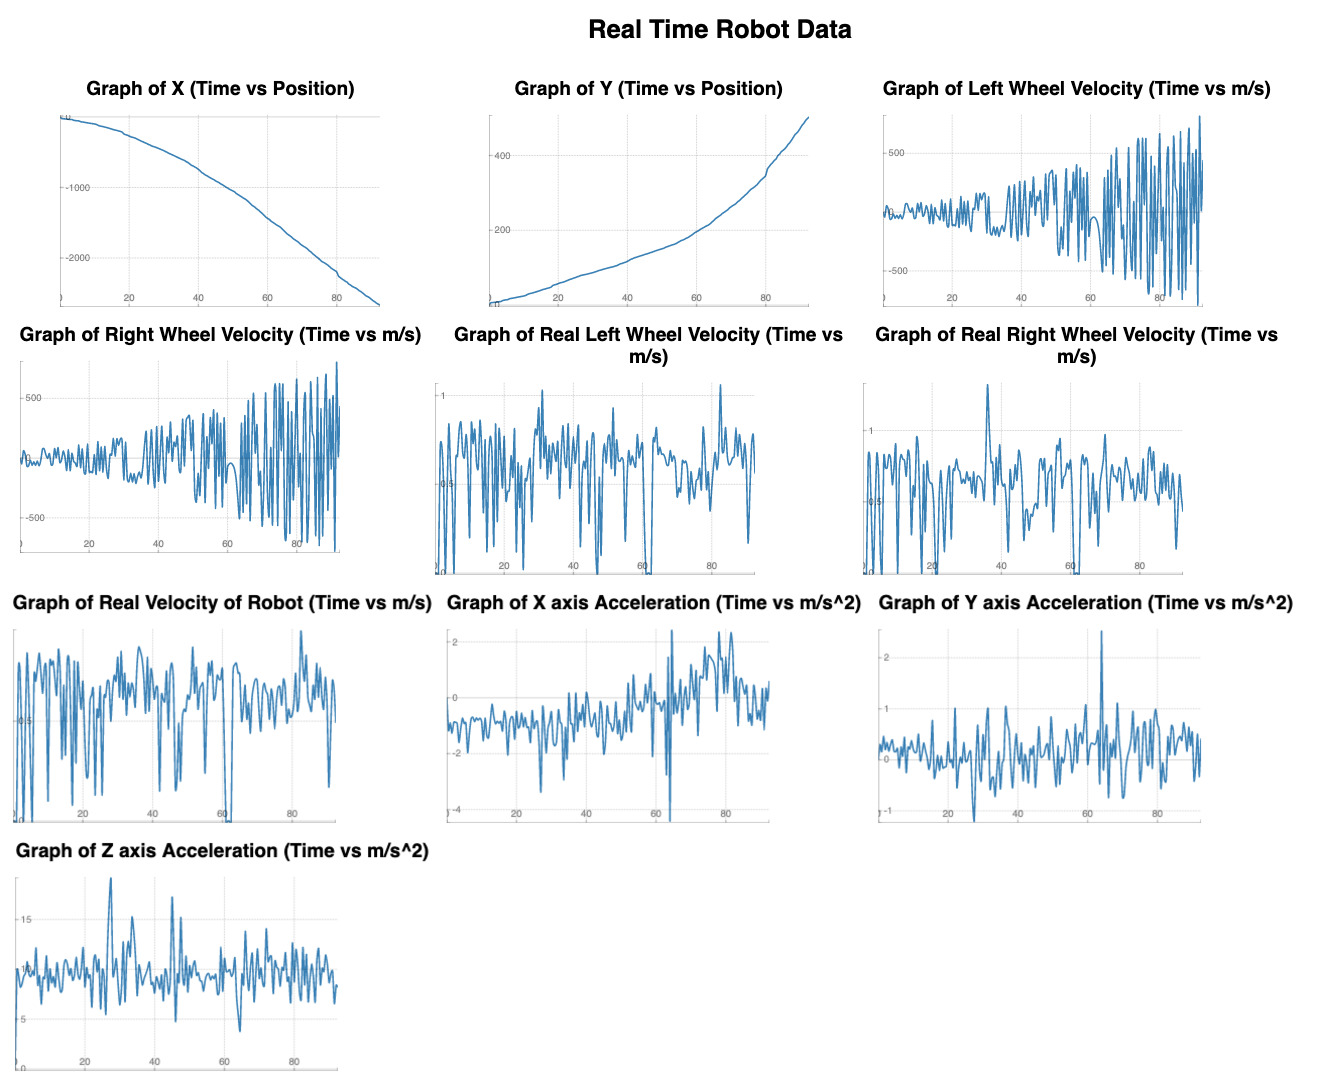
\includegraphics[width=6in]{14.jpg}
    \caption{Results of Steering to (200, 200)}  
    \label{6}
\end{figure}

\end{document}